\documentclass{article}
\usepackage{subcaption}
\usepackage[labelformat=parens,labelsep=quad, skip=3pt]{caption}
\usepackage{graphicx}
\usepackage[font=small,labelfont=bf]{caption}
\usepackage{geometry}

\geometry{
 a4paper,
 left=0mm,
 top=0mm,
 }

\begin{document}




\begin{figure}[htp]
 \centering
\begin{subfigure}{.33\textwidth}
 \caption{Atlantic O$_2$ - WOA (2009)}
 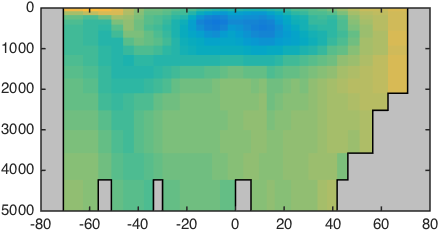
\includegraphics[width=0.95\linewidth]{../Separate_figures/OBSERVATIONS/Atlantic_o_an_profile.png}
 \label{fig:nutrients1}
\end{subfigure}%
\begin{subfigure}{.33\textwidth}
 \caption{Atlantic O$_2$ - cGEnIE}
 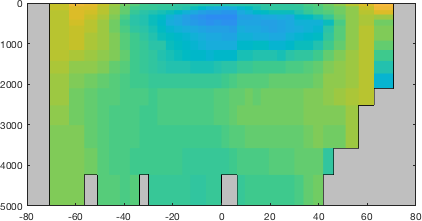
\includegraphics[width=0.95\linewidth]{../Separate_figures/BIOGEM/Atlantic_ocn_O2_profile.png}
 \label{fig:nutrients1}
\end{subfigure}%
\begin{subfigure}{.33\textwidth}
 \caption{Atlantic O$_2$ - EcoGEnIE}
 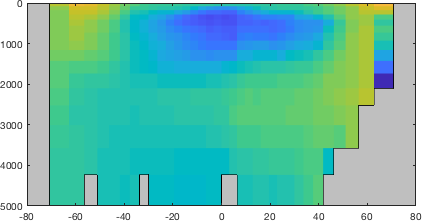
\includegraphics[width=0.95\linewidth]{../Separate_figures/ECOGEM/Atlantic_ocn_O2_profile.png}
 \label{fig:nutrients2}
\end{subfigure}
\begin{subfigure}{.33\textwidth}
 \caption{Indian O$_2$ - WOA (2009)}
 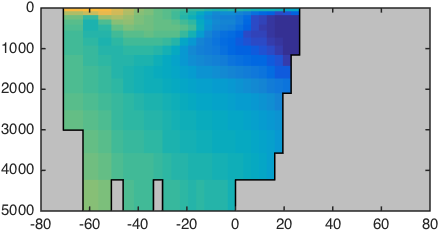
\includegraphics[width=0.95\linewidth]{../Separate_figures/OBSERVATIONS/Indian_o_an_profile.png}
 \label{fig:nutrients1}
\end{subfigure}%
\begin{subfigure}{.33\textwidth}
 \caption{Indian O$_2$ - cGEnIE}
 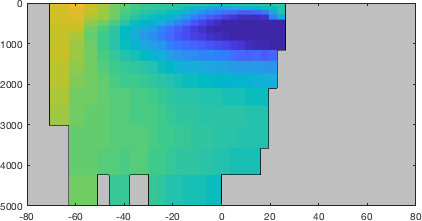
\includegraphics[width=0.95\linewidth]{../Separate_figures/BIOGEM/Indian_ocn_O2_profile.png}
 \label{fig:nutrients1}
\end{subfigure}%
\begin{subfigure}{.33\textwidth}
 \caption{Indian O$_2$ - EcoGEnIE}
 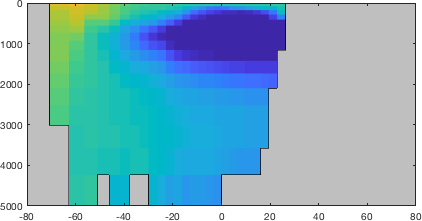
\includegraphics[width=0.95\linewidth]{../Separate_figures/ECOGEM/Indian_ocn_O2_profile.png}
 \label{fig:nutrients2}
\end{subfigure}
\begin{subfigure}{.33\textwidth}
 \caption{Pacific O$_2$ - WOA (2009)}
 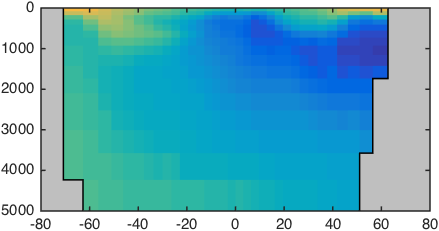
\includegraphics[width=0.95\linewidth]{../Separate_figures/OBSERVATIONS/Pacific_o_an_profile.png}
 \label{fig:nutrients1}
\end{subfigure}%
\begin{subfigure}{.33\textwidth}
 \caption{Pacific O$_2$ - cGEnIE}
 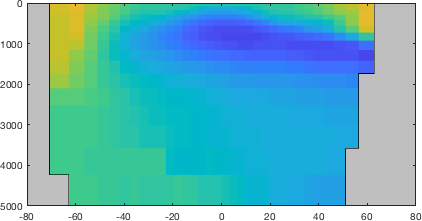
\includegraphics[width=0.95\linewidth]{../Separate_figures/BIOGEM/Pacific_ocn_O2_profile.png}
 \label{fig:nutrients1}
\end{subfigure}%
\begin{subfigure}{.33\textwidth}
 \caption{Pacific O$_2$ - EcoGEnIE}
 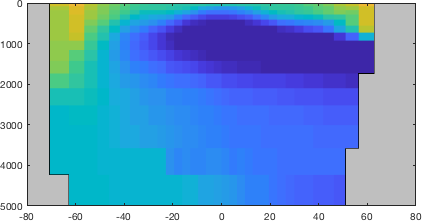
\includegraphics[width=0.95\linewidth]{../Separate_figures/ECOGEM/Pacific_ocn_O2_profile.png}
 \label{fig:nutrients2}
\end{subfigure}
\\[+0.2cm]
\begin{subfigure}{.5\textwidth}
 
\includegraphics[width=0.95\linewidth]{../Separate_figures/ECOGEM/ocn_O2_profile_clrbr.png}
\end{subfigure}
\end{figure}

\end{document}

\begin{figure}[htp]
 \centering
\begin{subfigure}{.33\textwidth}
 \caption{Atlantic ALK - GLODAPv2}
 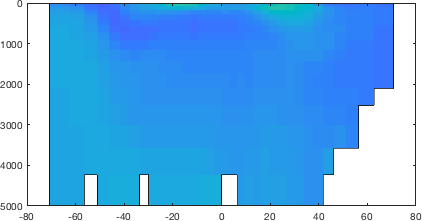
\includegraphics[width=0.95\linewidth]{../Separate_figures/OBSERVATIONS/Atlantic_TALK_profile.png}
 \label{fig:nutrients1}
\end{subfigure}%
\begin{subfigure}{.33\textwidth}
 \caption{Atlantic Alkalinity - cGEnIE}
 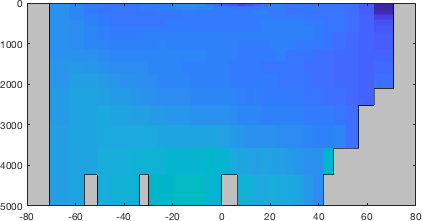
\includegraphics[width=0.95\linewidth]{../Separate_figures/BIOGEM/Atlantic_ocn_ALK_profile.png}
 \label{fig:nutrients1}
\end{subfigure}%
\begin{subfigure}{.33\textwidth}
 \caption{Atlantic Alkalinity - EcoGEnIE}
 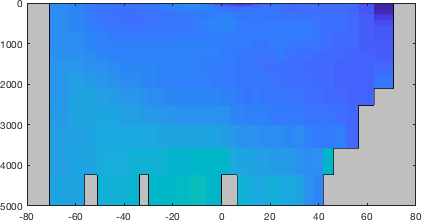
\includegraphics[width=0.95\linewidth]{../Separate_figures/ECOGEM/Atlantic_ocn_ALK_profile.png}
 \label{fig:nutrients2}
\end{subfigure}
\begin{subfigure}{.33\textwidth}
 \caption{Indian ALK - GLODAPv2}
 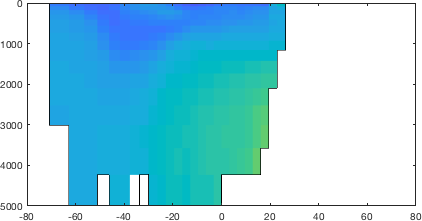
\includegraphics[width=0.95\linewidth]{../Separate_figures/OBSERVATIONS/Indian_TALK_profile.png}
 \label{fig:nutrients1}
\end{subfigure}%
\begin{subfigure}{.33\textwidth}
 \caption{Indian Alkalinity - cGEnIE}
 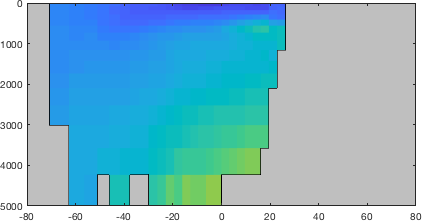
\includegraphics[width=0.95\linewidth]{../Separate_figures/BIOGEM/Indian_ocn_ALK_profile.png}
 \label{fig:nutrients1}
\end{subfigure}%
\begin{subfigure}{.33\textwidth}
 \caption{Indian Alkalinity - EcoGEnIE}
 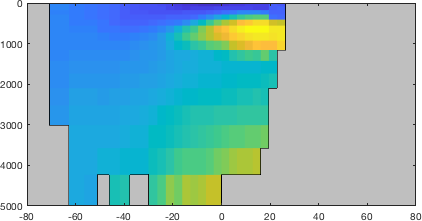
\includegraphics[width=0.95\linewidth]{../Separate_figures/ECOGEM/Indian_ocn_ALK_profile.png}
 \label{fig:nutrients2}
\end{subfigure}
\begin{subfigure}{.33\textwidth}
 \caption{Pacific ALK - GLODAPv2}
 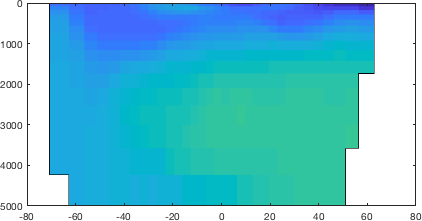
\includegraphics[width=0.95\linewidth]{../Separate_figures/OBSERVATIONS/Pacific_TALK_profile.png}
 \label{fig:nutrients1}
\end{subfigure}%
\begin{subfigure}{.33\textwidth}
 \caption{Pacific Alkalinity - cGEnIE}
 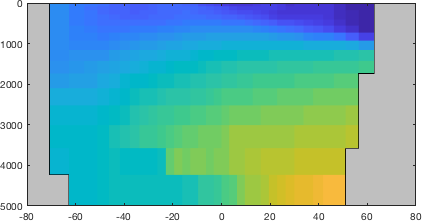
\includegraphics[width=0.95\linewidth]{../Separate_figures/BIOGEM/Pacific_ocn_ALK_profile.png}
 \label{fig:nutrients1}
\end{subfigure}%
\begin{subfigure}{.33\textwidth}
 \caption{Pacific Alkalinity - EcoGEnIE}
 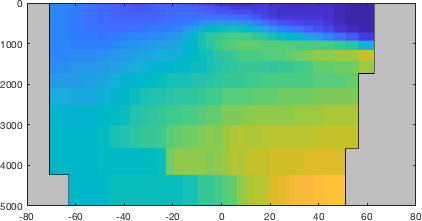
\includegraphics[width=0.95\linewidth]{../Separate_figures/ECOGEM/Pacific_ocn_ALK_profile.png}
 \label{fig:nutrients2}
\end{subfigure}
\\[+0.2cm]
\begin{subfigure}{.5\textwidth}
 
\includegraphics[width=0.95\linewidth]{../Separate_figures/ECOGEM/ocn_ALK_profile_clrbr.png}
\end{subfigure}
\end{figure}


